% !TEX root = main.tex

\documentclass[twocolumn]{article}

% Required packages
\usepackage{graphicx}  % For images
\usepackage{amsmath, amssymb} % Math symbols
\usepackage[external]{gnuplottex}
\usepackage{titlesec} % Formatting sections
\usepackage{fancyhdr} % Header and Footer customization
\usepackage{abstract} % Abstract formatting
\usepackage{titling} % Title customization
\usepackage{authblk} % Author affiliations
\usepackage{babel} % For figure legends
\usepackage{siunitx} % For SI units
\usepackage{hyperref} % For hyperlinks in the PDF
\usepackage{lipsum} 

\usepackage{blindtext} % Package to generate dummy text throughout this template 
\usepackage[sc]{mathpazo} % Use the Palatino font
\usepackage[T1]{fontenc} % Use 8-bit encoding that has 256 glyphs
\linespread{1.05} % Line spacing - Palatino needs more space between lines
\usepackage{microtype} % Slightly tweak font spacing for aesthetics
\usepackage{float}
\usepackage[a4paper, margin=1in,hmarginratio=1:1,top=15mm,left=12mm,bottom=25mm,columnsep=15pt]{geometry} % Document margins
\usepackage{enumitem} % Customized lists
\setlist[itemize]{noitemsep} % Make itemize lists more compact
\usepackage{abstract} % Allows abstract customization
\renewcommand{\abstractnamefont}{\normalfont\bfseries} % Set the "Abstract" text to bold
\renewcommand{\abstracttextfont}{\normalfont\small\itshape} % Set the abstract itself to small italic text
\usepackage{titlesec} % Allows customization of titles
\renewcommand\thesection{\Roman{section}} % Roman numerals for the sections
\renewcommand\thesubsection{\roman{subsection}} % roman numerals for subsections
\titleformat{\section}[block]{\large\scshape\centering}{\thesection.}{1em}{} % Change the look of the section titles
\titleformat{\subsection}[block]{\large}{\thesubsection.}{1em}{} % Change the look of the section titles


% Define Cover Page
\newcommand{\coverpage}{
    \begin{titlepage}
        \centering
        \vspace*{2cm}
        {\Huge \textbf{Quantum-inspired machine learning on a quantum computer}}\\[1cm]
        {\Large João Guilherme}\\[0.5cm]
        {\large Instituto Superior Técnico, Department of Physics}\\[2cm]
        {\large \today}\\[3cm]
        \vfill
        \begin{abstract}
            This document presents...
        \end{abstract}
        \vfill
    \end{titlepage}
}



% Begin document
\begin{document}

% Insert Cover Page
\coverpage

% Example Section
\section{Introduction}
This is an example introduction.

\section{Encoding of the data}
\subsection{Gram matrix encoding}

Considering a column vector with data, $u$, the gram encoding is given by:
$$
\rho = \frac{uu^T}{\sqrt{\| uu^T \|}} = \frac{uu^T}{Tr(uu^T)}
$$

\begin{figure}
    \centering
    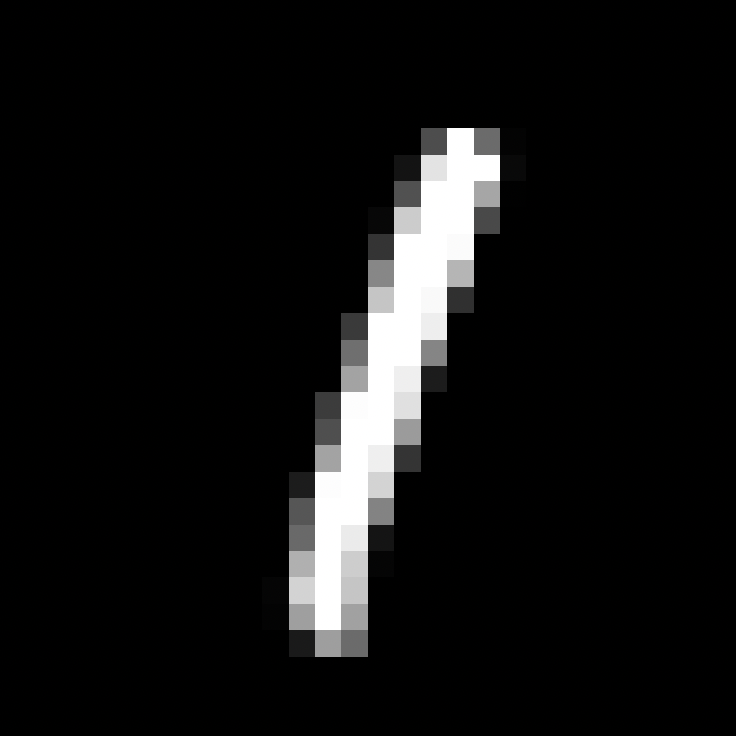
\includegraphics[width=\linewidth]{figures/nmist_1_data.png}
    \caption{Image from the nmist dataset of the number 1}
    \label{fig:dataset_one}
\end{figure}

\begin{figure}
    \centering
    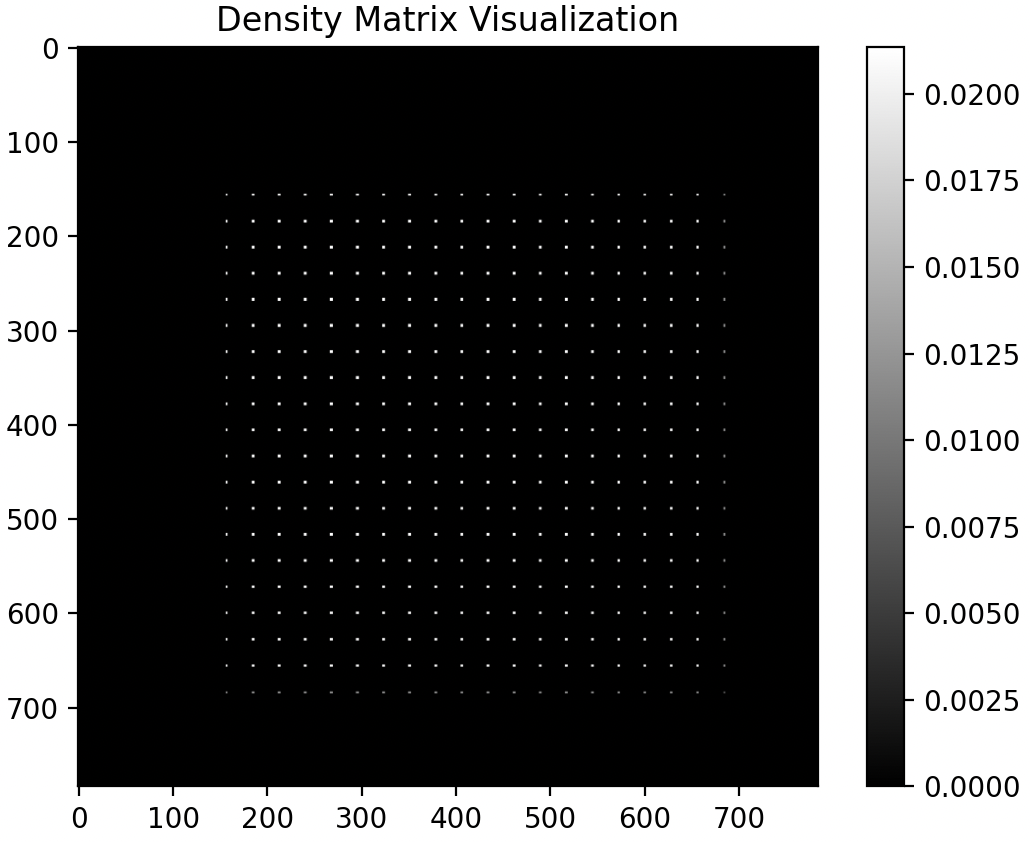
\includegraphics[width=\linewidth]{figures/density_matrix_nmist_one.png}
    \caption{Density matrix of the image from the dataset}
    \label{fig:enter-label}
\end{figure}

How to decode the image:

\section{Radial Basis Function Model}
Each point ($x_n$, $y_n$) $\in D$ influences the hypotesis, $h(x)$, based on $\| x - x_n \|$ (a near point affects more than a far away point)

Standard form:
$$
h(x) = \sum_{n=1} ^N w_n\exp\left({-\gamma\| x - x_n \|^2}\right)
$$

Radial - depends on $\| x - x_n \|$

Basis Function - in this case the basis function is $\exp{}$, but we could use other symmetric function

\textbf{The learning algorithm:}
Based on $D = (x_1,y_1), (x_2, y_2),...,(x_n,y_n)$

We want to set the in sample error to zero: $E_{in} = 0 \iff h(x_n) = y_n$, so we get:
$$
\sum_{m = 1}^N w_m\exp{\left( -\gamma\|x_n - x_m \|^2\right)} = y_n
$$
Translating into matrix form:

\[
\Phi \mathbf{w} = \mathbf{y}, \quad \text{where} \quad \Phi_{n,m} = \exp\left( -\gamma\|x_n - x_m\|^2 \right)
\]

To exist a solution, $\Phi$ must be invertible, and the solution is given by $w = \Phi^{-1} y$ - exact interpolation 

The $\gamma$ factor controlls the size of the gaussian functions, and will be chosen optmimally.

\textbf{Classification using RBF:}
$$
h(\textbf{x}) = \text{sign}\left(\sum_{n=1}^N w_n\exp\left(-\gamma\|x - x_n \|^2\right)\right) = \text{sign}(s)
$$

We will use something similar to linear regression classificaiton

s = $\sum_{n=1}^N w_n\exp\left(-\gamma\|x - x_n \|^2\right)$

\textbf{The learning algorithm:}
Minimize the error function: $(s - y)^2$ on the training set $D$, with $y \in \{-1, 1\}$ , this is a form of least squares regression.

\textbf{RBF with K centers}
$N$ parameters: $w_1, w_2, ..., w_N$ based on $N$ data points, can be reduced to using $K$ centers, $\mu_1, \mu_2, ..., \mu_K$ with $K \ll N$, so the new hypothesis is:
$$
h(x) = \sum_{k=1}^K w_k\exp\left(-\gamma\|x - \mu_k \|^2\right)
$$

There are then two questions:
1. How to choose the centers?
2. How to choose the weights?

\subsection{Choosing the centers}
The idea is to, instead of having a center for each data point, we will cluster the data points around a center, and we choose the centers by minimizing the distance between the data point, $x_n$, and the closest center, $\mu_k$. For this clustering, we will use K-Means clustering:

Split the data into $K$ and minimize our objective function $\sum_{k=1}^K\sum_{x_n \in S_k}\|x_n - \mu_k\|^2$.

But there is a problem! This is an NP-Hard problem.

To solve this problem we will use the Lloyd's algorithm to iteratively minimize the objective function. The algorithm is as follows:
$$
\mu_k = \frac{1}{|S_k|}\sum_{x_n \in S_k} x_n
$$

$$
S_k = \{ x_n \in D | \|x_n - \mu_k\| \leq \|x_n - \mu_j\|, j \neq k \}
$$

Both of this steps reduce the objective function, and we can repeat this until convergence, and we will reach a local minimum. 
To run this algorithm, we need to run the algorithm for a number of times, and choose the best solution.

\begin{figure}
    \centering
    \begin{gnuplot}[scale=0.6, terminal=pdf]
set title "3D Gaussian Function"
set xlabel "x"
set ylabel "y"
set zlabel "z"
set hidden3d
set view 60, 80
set isosamples 50, 50
set xrange [-5:5]
set yrange [-5:5]

# Parameters for the Gaussian
sigma = 1.0
mu_x = 0.0
mu_y = 0.0

# 2D Gaussian Function
gaussian(x, y) = exp(-((x - mu_x)**2 + (y - mu_y)**2) / (2 * sigma**2))

splot gaussian(x, y) with lines palette
\end{gnuplot}
    \caption{Caption}
    \label{fig:asd}
\end{figure} 

% Example Gnuplot
\begin{figure}
    \centering
    \begin{gnuplot}[scale=0.6, terminal=pdf]
set xlabel "X-axis"
set ylabel "Y-axis"
plot sin(x)
\end{gnuplot}
        
    \caption{Example Figure}
    \label{fig:gnuplot_example}
\end{figure}

\lipsum[1-20]

\cite{Cruzeiro2024}


\bibliography{references}{}
\bibliographystyle{plain}

\end{document}